\documentclass[]{book}
\usepackage{lmodern}
\usepackage{amssymb,amsmath}
\usepackage{ifxetex,ifluatex}
\usepackage{fixltx2e} % provides \textsubscript
\ifnum 0\ifxetex 1\fi\ifluatex 1\fi=0 % if pdftex
  \usepackage[T1]{fontenc}
  \usepackage[utf8]{inputenc}
\else % if luatex or xelatex
  \ifxetex
    \usepackage{mathspec}
  \else
    \usepackage{fontspec}
  \fi
  \defaultfontfeatures{Ligatures=TeX,Scale=MatchLowercase}
\fi
% use upquote if available, for straight quotes in verbatim environments
\IfFileExists{upquote.sty}{\usepackage{upquote}}{}
% use microtype if available
\IfFileExists{microtype.sty}{%
\usepackage{microtype}
\UseMicrotypeSet[protrusion]{basicmath} % disable protrusion for tt fonts
}{}
\usepackage[margin=1in]{geometry}
\usepackage{hyperref}
\hypersetup{unicode=true,
            pdftitle={Planning Tool Guidance},
            pdfauthor={Project Big Life},
            pdfborder={0 0 0},
            breaklinks=true}
\urlstyle{same}  % don't use monospace font for urls
\usepackage{natbib}
\bibliographystyle{apalike}
\usepackage{longtable,booktabs}
\usepackage{graphicx,grffile}
\makeatletter
\def\maxwidth{\ifdim\Gin@nat@width>\linewidth\linewidth\else\Gin@nat@width\fi}
\def\maxheight{\ifdim\Gin@nat@height>\textheight\textheight\else\Gin@nat@height\fi}
\makeatother
% Scale images if necessary, so that they will not overflow the page
% margins by default, and it is still possible to overwrite the defaults
% using explicit options in \includegraphics[width, height, ...]{}
\setkeys{Gin}{width=\maxwidth,height=\maxheight,keepaspectratio}
\IfFileExists{parskip.sty}{%
\usepackage{parskip}
}{% else
\setlength{\parindent}{0pt}
\setlength{\parskip}{6pt plus 2pt minus 1pt}
}
\setlength{\emergencystretch}{3em}  % prevent overfull lines
\providecommand{\tightlist}{%
  \setlength{\itemsep}{0pt}\setlength{\parskip}{0pt}}
\setcounter{secnumdepth}{5}
% Redefines (sub)paragraphs to behave more like sections
\ifx\paragraph\undefined\else
\let\oldparagraph\paragraph
\renewcommand{\paragraph}[1]{\oldparagraph{#1}\mbox{}}
\fi
\ifx\subparagraph\undefined\else
\let\oldsubparagraph\subparagraph
\renewcommand{\subparagraph}[1]{\oldsubparagraph{#1}\mbox{}}
\fi

%%% Use protect on footnotes to avoid problems with footnotes in titles
\let\rmarkdownfootnote\footnote%
\def\footnote{\protect\rmarkdownfootnote}

%%% Change title format to be more compact
\usepackage{titling}

% Create subtitle command for use in maketitle
\providecommand{\subtitle}[1]{
  \posttitle{
    \begin{center}\large#1\end{center}
    }
}

\setlength{\droptitle}{-2em}

  \title{Planning Tool Guidance}
    \pretitle{\vspace{\droptitle}\centering\huge}
  \posttitle{\par}
    \author{Project Big Life}
    \preauthor{\centering\large\emph}
  \postauthor{\par}
      \predate{\centering\large\emph}
  \postdate{\par}
    \date{2019-07-29}

\usepackage{booktabs}
\usepackage{amsthm}
\makeatletter
\def\thm@space@setup{%
  \thm@preskip=8pt plus 2pt minus 4pt
  \thm@postskip=\thm@preskip
}
\makeatother

\begin{document}
\maketitle

{
\setcounter{tocdepth}{1}
\tableofcontents
}
\chapter{Welcome to Project Big Life's Planning
Tool}\label{welcome-to-project-big-lifes-planning-tool}

\emph{TO DO: Insert the image for the PBL planning tool}

\subsection{What is the Project Big Life Planning
Tool}\label{what-is-the-project-big-life-planning-tool}

\emph{To do: Develop video showcasing the platform including what it is
and why someone should use the platform}

\subsection{Who made the Project Big Life Planning
Tool?}\label{who-made-the-project-big-life-planning-tool}

The Project Big Life Planning Tool was developed by the Project Big Life
Team. The Project Big Life Team is part of the ICES. The below video
explains what ICES is.

\begin{verbatim}
## PhantomJS not found. You can install it with webshot::install_phantomjs(). If it is installed, please make sure the phantomjs executable can be found via the PATH variable.
\end{verbatim}

\chapter{Introduction}\label{introduction}

The Project Big Life Planning Tool was developed in order to support
health professionals: research, plan, develop, and evaluate
evidence-based health interventions.

For instance Project Big Life Planning Tool helps:

\begin{itemize}
\tightlist
\item
  Public health professionals: assess the impact of preventative
  interventions that target health behaviours
\item
  Health planners: assess the need for palliative care
\end{itemize}

\textbf{What types of questions can it answer?}

The Project Big Life Planning Tool can answer the following types of
questions:

\begin{itemize}
\tightlist
\item
  What is the burden of smoking on life expectancy?
\item
  How many deaths would be prevented if everyone met their daily
  exercise requirements?
\end{itemize}

\textbf{How does it work?}

\begin{itemize}
\item
  This tool provides health planners with access to multivariable
  predictive risk algorithms, created and housed by the Project Big Life
  Team.
\item
  The multivariable predictive risk algorithms use distinct
  characteristics and health profiles of groups of people to assess the
  risk of a health outcome (e.g.~Life Expectancy).
\item
  The multivariable predictive risk algorithms are developed and
  validated using data routinely collected by Statistics Canada and
  provincial health agencies, and the algorithms have been published in
  various journals.
\item
  More information about multivariable predictive risk algorithms can be
  found in the key concepts (Chapter \ref{keyconcepts}).
\end{itemize}

\textbf{Why should I used it?}

\begin{itemize}
\item
  It is \textbf{easy} and \textbf{flexible} to use.

  \begin{itemize}
  \tightlist
  \item
    The user only needs to upload their data and choose which
    calculation to run.
  \item
    It can be used to assess the future risk of a health outcome.
  \item
    It can be used to assess the effectiveness of different intervention
    scenarios (e.g.~policy) on a health outcome.
  \end{itemize}
\item
  It generates \textbf{accurate} predictions.

  \begin{itemize}
  \tightlist
  \item
    It can be used to accurately assess the risk of a health outcome in
    populations that were not used in its developement, and groups of
    people that account for only a fraction of the population.
  \end{itemize}
\item
  It is \textbf{private}.

  \begin{itemize}
  \tightlist
  \item
    Loaded data remains on your computer and is not uploaded or sent
    anywhere.
  \end{itemize}
\end{itemize}

\chapter{Getting Started}\label{getting-started}

To help you get started quickly with Project Big Life's Planning Tool,
we built a Tutorial directly onto the platform.

The tutorial takes you through step-by-step how to use Project Big
Life's Planning Tool. The tutorial will not explain the steps in detail
(Chapter \ref{howto}) nor will it provide reference material (Chapter
\ref{glossary}), but it will give you an understanding of how easy it is
to use the Planning Tool!

\textbf{To access the tutorial}, go onto Project Big Life's Planning
Tool (\url{http://policy.projectbiglife.ca/}) and click on the Tutorial
button in the top right corner!

\begin{center}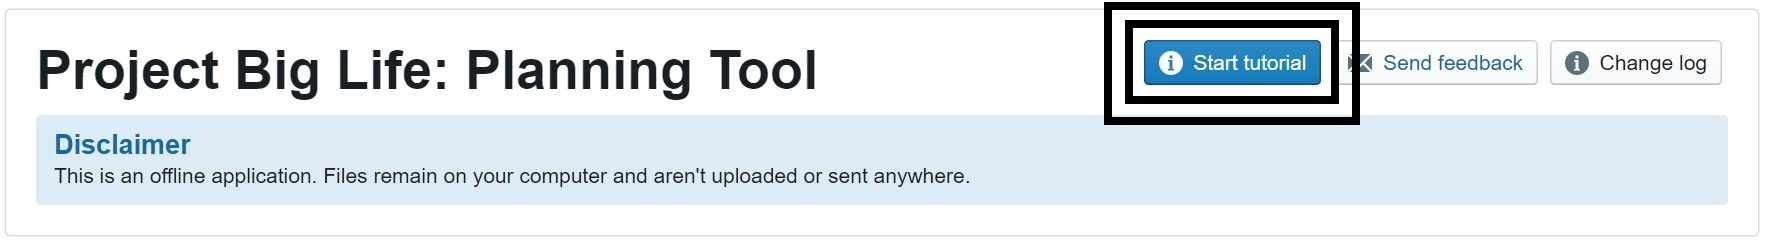
\includegraphics{Tutorial Button} \end{center}

\chapter{How To}\label{howto}

These guides will cover the topics covered in the tutorial but in
greater detail.

\begin{itemize}
\tightlist
\item
  Customize data
\item
  Load data
\item
  Select calculation
\item
  Filter data
\item
  Stratify data
\item
  Run scenarios: Intervention and Cause-deleted
\item
  Calculate results
\item
  Visualize data (TBD)
\item
  Export data (TBD)
\item
  Resolve error messages (TBD)
\end{itemize}

\section{Customize Data}\label{customize-data}

Prior to using the Project Big Life Planning Tool you may want to
manipulate your data set. Reasons include: custom filter(s) and/or
custom stratification(s).

Data manipulation can occur on any programming software: R, SAS, STATA,
etc, as long as you output your data set as a `.csv' file.

An example of customizing your data set is converting the variable: Body
Mass Index (CCHS 2013 variable HWTGBMI) from a continuous variable into
four distinct categories:

\begin{itemize}
\tightlist
\item
  Underweight: BMI less then 18.5
\item
  Normal or Healthy Weight: BMI of 18.5 to 24.9
\item
  Overweight: BMI of 25.0 to 29.9
\item
  Obese: BMI greater or equal to 30.0
\end{itemize}

\textbf{Steps}

The following shows R code that would be used to create these
stratifications:

\begin{enumerate}
\def\labelenumi{\arabic{enumi}.}
\item
  Convert observations ``Not stated'' from 999.99 to N/A

\begin{verbatim}
data[data == 999.99] <- NA
\end{verbatim}
\item
  Load the R package dpylr. This package is used for data manipulation.

\begin{verbatim}
library(dpylr)
\end{verbatim}
\item
  Create a new column that contains four categories for BMI

\begin{verbatim}
data$newcolumn <- cut(data$HWTGBMI, breaks = c(0,18.5,25,30,Inf),  labels=c("Underweight", "Healthy", "Overweight", "Obese")
\end{verbatim}
\item
  The output will be your data set + a new column with the corresponding
  category (``Underweight'', ``Healthy'', ``Overweight'', ``Obese'') for
  that individual.
\end{enumerate}

\begin{verbatim}
    HWTGBMI   newcolumn
  1   22.68     Healthy
  2   26.99  Overweight
  3      NA        <NA>
  4   34.44       Obese
  5   23.77     Healthy
  6   17.23 Underweight
\end{verbatim}

This new column can be used with the Project Big Life Planning Tool for
filtering or stratification.

\section{Load data}\label{load-data}

Only one data set can be used on the platform for each calculation; a
calculation cannot be preformed across multiple data sets.

\textbf{Note:} Data sets loaded to the Project Big Life Planning Tool
remains on your computer and is not uploaded or sent anywhere.

There are two options for your data: use a sample file or load your own
file.

\textbf{Note:} The Project Big Life Planning Tool can currently only
support .csv data files from the 2013/2014 Canadian Community Health
Survey. Both the PUMF and Shared 2013/2014 Canadian Community Health
Survey files are accepted. \emph{Need to confirm the geography
variables}

\begin{itemize}
\tightlist
\item
  More information on the Canadian Community Health Survey and the types
  of accepted data can be found in Key concepts (Chapter
  \ref{keyconcepts}) - ``Data and Sample Files''.
\end{itemize}

\subsection{Load sample files}\label{load-sample-files}

If you don't have your own data or want to explore the platform's
capabilities before using your data, you can use the sample files on the
Project Big Life Planning Tool. There are \textbf{X} sample files you
may use:

\begin{itemize}
\item
  MockPUMF2013.csv is a sub-sample of the Public Use Microdata File from
  the 2013 Canadian Community Health Survey. This file has all the
  required and recommended variables.
\item
  SmallMockPUMF2013.csv \emph{TO FIGURE OUT WHAT IT INCLUDES}
\end{itemize}

\textbf{Steps}

\begin{enumerate}
\def\labelenumi{\arabic{enumi}.}
\tightlist
\item
  Click on the file name under ``Sample files'' to select it.
\end{enumerate}

\subsection{Load your own file}\label{load-your-own-file}

\textbf{Steps}

\begin{enumerate}
\def\labelenumi{\arabic{enumi}.}
\item
  Click the \textbf{Browse} button under ``Select a file to use in
  calculations''.
\item
  Locate the file on your computer, select, and open.
\end{enumerate}

\begin{itemize}
\item
  If the loaded file has all of the variables required and recommended
  for calculation, you will be able to continue with the planning tool.
\item
  If the loaded file does \textbf{not} have all the variables
  \textbf{required} for the calculation you will not be able to continue
  with the planning tool.
\item
  If the loaded file does \textbf{not} have all the variables
  \textbf{recommended} for calculation you will be able to continue with
  the planning tool, however the calculations may be less accurate.
\end{itemize}

\section{Select calculation}\label{select-calculation}

There are two general types of calculations: summary measures and by row
measures.

\begin{itemize}
\item
  \textbf{Summary measures:} When selected, the result will be a single measure for
the entire dataset. For instance when Summary Measure - Life Expectancy
(Summary Measure) is selected the result is a single life expectancy for
the given for the population.
\item
  \textbf{By row measures:} When selected, the result will be the measurement for
each individual (e.g.~row) in the dataset.
\end{itemize}

Summary measures must be selected for calculations that have
stratifications, intervention scenarios, and cause-deleted scenario.

\textbf{Steps}

\begin{enumerate}
\def\labelenumi{\arabic{enumi}.}
\tightlist
\item
  Check the box beside the calculation's name under ``Calculations'' to
  select it. A single calculation or multiple calculations may be
  selected.
\end{enumerate}

\begin{itemize}
\tightlist
\item
  Once selected the name(s) of the calculation(s) will appear to the
  right of ``Calculations''.
\end{itemize}

More details of what the calculations are and how they are preformed can
be found in key concepts (Chapter \ref{keyconcepts}) - ``Calculations''.

\section{Filter data}\label{filter-data}

Use filters when you want to analyze only a subset of your data.

\textbf{Steps}

\begin{enumerate}
\def\labelenumi{\arabic{enumi}.}
\item
  Click on the \textbf{+ New} button under ``Filters''.
\item
  Select the variable that you want to filter on by typing its variable
  name into the ``search variables'' text bar.
\item
  Filter \textbf{in} the categories/levels within the variable by:
\end{enumerate}

\begin{itemize}
\item
  \textbf{Categorical:} Clicking on the ``Search categories''" text bar.
  Scroll and select the category you want to \textbf{keep} in your data.
  Repeat this step to add additional categories.
\item
  \textbf{Continous:} Click the ``cycle button'' found under the
  variable you have selected. Two new boxes will appear.

  \begin{itemize}
  \tightlist
  \item
    Select the minimum value for your subset data in the box on the left
    by typing the values or using the arrows.
  \item
    Select the maximum value for your subset data in the box on your
    right by typing the value or using the arrows.
  \end{itemize}
\end{itemize}

\begin{enumerate}
\def\labelenumi{\arabic{enumi}.}
\setcounter{enumi}{3}
\tightlist
\item
  To add another filter repeat the steps above. A maximum of three
  filters are recommended to maintain statistical power (added filters
  reduce sample sizes and reduces statistical power).
\end{enumerate}

\begin{itemize}
\tightlist
\item
  Once selected, the name(s) of the filtered variable(s) will appear to
  the right of ``Filters''.
\end{itemize}

You are able to filter on all types of variables: required for
calculation, recommended for calculation, and ignore variables (includes
customized variables).

\subsection{Remove a filter}\label{remove-a-filter}

\begin{itemize}
\item
  To remove a filter entirely, click on the trash can beside the
  variable you want to delete.
\item
  To remove a level within a filtered variable - categorical, click on
  the `x' beside the variable level.
\end{itemize}

\section{Stratify data}\label{stratify-data}

Use stratifications when you want to get a result for multiple strata
(levels or classes).

A summary measure must be selected for stratifications, as only a
summary measure will be outputted for each strata. By row measurements
may also be selected but they will not be stratified.

\textbf{Steps}

\begin{enumerate}
\def\labelenumi{\arabic{enumi}.}
\item
  Click the box beside either ``Life Expectancy (Summary)'' or ``Deaths
  (Five Years)'' under the ``Calculation'' drop down.
\item
  Select the variables you want to stratify on under the
  ``Stratifications'. You are only able to stratify on categorical
  variables.
\item
  To add another variable for stratification repeat the steps above. A
  maximum of 3 stratifications are recommended to maintain statistical
  power (added strata reduce strata sample size and reduces statistical
  power).
\end{enumerate}

\begin{itemize}
\tightlist
\item
  Once selected, the name(s) of the stratified variable(s) will appear
  to the right of ``Stratifications''.
\end{itemize}

You are able to stratify on all types of categorical variables: required
for calculation, recommended for calculation, and ignore variables
(includes customized variables).

\subsection{Remove a stratification}\label{remove-a-stratification}

\begin{itemize}
\tightlist
\item
  To remove a stratification variable click on the `x' beside the
  variable level.
\end{itemize}

\section{Run scenarios}\label{run-scenarios}

Scenarios can be used to predict the health outcomes when unhealthy
behaviours:

\begin{itemize}
\tightlist
\item
  are modified in the population: \textbf{Intervention}, or
\item
  were never present in the population: \textbf{Cause-deleted}
\end{itemize}

Scenarios can be used to inform potential health policies or programs.

\subsection{Intervention scenarios}\label{intervention-scenarios}

Interventions provide you with the ability to customize the scenarios.
For example you can answer the questions:

\begin{itemize}
\tightlist
\item
  what if we only had 15\% of the population smoked rather then the
  current 20\%?
\item
  what if everyone increased their physical activity by 10\%?
\item
  what if everyone ate 4 fruit servings each day?
\item
  what if everyone drank 2 fewer drinks per week?
\end{itemize}

These intervention scenarios allow you to predict and compare the
effectiveness of policies.

There are 3 types of intervention scenarios that you can select:

\begin{itemize}
\tightlist
\item
  \textbf{Absolute:} each individual in the population \textbf{changes}
  their health behaviour \textbf{by a value of x}.
\item
  \textbf{Relative:} each individual in the population \textbf{changes}
  their health behaviour \textbf{by a ratio of y}.
\item
  \textbf{Target:} each individual in the population \textbf{has a set
  value of z.}
\end{itemize}

More information on the specifics of each type of intervention scenario
and how they are calculated can be found in Key Concepts (Chapter
\ref{keyconcepts}) - ``Scenarios: Interventions''.

\textbf{Steps}

\begin{enumerate}
\def\labelenumi{\arabic{enumi}.}
\item
  Click the box beside either ``Life Expectancy (Summary)'' under the
  ``Calculation'' drop down.
\item
  Check the button beside: ``Intervention'' under the ``Scenario'' drop
  down.
\item
  Click on the health behaviour you want to modify: e.g.~Diet.
\end{enumerate}

\begin{itemize}
\tightlist
\item
  A drop down menu of all the possible variables of that health
  behaviour you can modify will appear.
\end{itemize}

\begin{enumerate}
\def\labelenumi{\arabic{enumi}.}
\setcounter{enumi}{3}
\tightlist
\item
  Click the box beside the variable you want to modify: e.g.~Daily
  consumption - fruit - (D).
\end{enumerate}

\begin{itemize}
\tightlist
\item
  A drop down menu of the scenario types: absolute, relative, and
  target, will appear.
\end{itemize}

\begin{enumerate}
\def\labelenumi{\arabic{enumi}.}
\setcounter{enumi}{4}
\item
  Check the button beside the type of intervention you want to modify:
  e.g.~Target.
\item
  Use the arrows beside the the text box: ``Decrease by'' or ``Increase
  by'' to add the value you are modifying: e.g.~The value of 4 is used
  for the scenario what if everyone ate 4 fruit servings each day?
\end{enumerate}

Multiple health behaviours and variables within the health behaviours
can be selected for a single calculation.

\begin{itemize}
\tightlist
\item
  Once selected, the name(s) of the health behaviour(s) that have been
  selected for the intervention will appear to the right of
  ``Scenario''.
\end{itemize}

\subsection{Cause-deleted scenarios}\label{cause-deleted-scenarios}

Cause-deleted scenarios provide you with the ability to see the best
case scenario for the population. For example:

\begin{itemize}
\tightlist
\item
  what if no one in the population ever smoked?
\item
  what if everyone in the population met their recommended physical
  activity levels (3.00 METs/week)?
\end{itemize}

More information on cause-deleted calculations and how they are
calculated can be found in key concepts (\emph{Chapter
\ref{keyconcepts}}) - ``Scenarios: Cause-deleted''.

\textbf{Steps}

\begin{enumerate}
\def\labelenumi{\arabic{enumi}.}
\item
  Click the box beside either ``Life Expectancy (Summary)'' under the
  ``Calculation'' drop down.
\item
  Check the button beside: ``Cause-deleted'' under the ``Scenario'' drop
  down.
\item
  Check the box beside the health behaviour that you want to have a
  cause-deleted calculation.
\end{enumerate}

Multiple health behaviours can be selected for a single calculation.

\section{Calculate results}\label{calculate-results}

\begin{enumerate}
\def\labelenumi{\arabic{enumi}.}
\tightlist
\item
  Name your calculation in the text box: Calculation name.
\end{enumerate}

\begin{itemize}
\tightlist
\item
  Be specific when naming the calculation as it will make it easier to
  distinguish after running multiple calculations.
\end{itemize}

\textbf{Note:} the larger the data set is the longer the calculations
will take. Depending on the size of the data set and the type of
calculation being preformed it could take an hour or more.

\section{Visualize Data}\label{visualize-data}

\emph{TBD: Need plots on the platform to work through the steps below} -
export - create your own(?)

\section{Download results}\label{download-results}

Click on the \textbf{Download results} button under the \textbf{Results}
section.

Select which calculations you'd like to download.

\emph{To Do: Screenshot of all the calculation options once the platform
is fixed.}

\section{Resolve warning or error
messages}\label{resolve-warning-or-error-messages}

There are different types of warning and error messages that may appear.

Below describes some of the messages that are likely to occur and steps
to resolve them.

\emph{Waiting for the branch with the error messages to be finalized and
merged}

\subsection{Invalid category}\label{invalid-category}

\subsection{Out of range}\label{out-of-range}

``Out of range'' is when there are observation(s) in the data set that
are not is beyond the limit of

\subsection{Not a number}\label{not-a-number}

\subsection{Sample size is too small}\label{sample-size-is-too-small}

\chapter{Applications}\label{applications}

This chapter provides you with examples of how Project Big Life's
Planning Tool can be used in your day-to-day operations. The examples
will cover:

\begin{itemize}
\tightlist
\item
  analyses that can be included in a health status report,
\item
  a national policy: What if Canada biked like the Dutch?
\item
  a local policy: turning Ottawa into the healthiest Canadian region
\item
  a
\end{itemize}

\section{Health Status Report}\label{health-status-report}

In this example we will highlight statistics that could reported in
health status reports. Health status reports are a way to report the
health state for a population and the factors that influence the
population's health. Information from health status reports are used to
inform policy, planning, and resource allocation.

In this example we will calculate:

\begin{itemize}
\tightlist
\item
  The predicted number of deaths by strata
\item
  The impact of eliminating unhealthy behaviours on life expectancy
\end{itemize}

For this example we will focus on the population of Alberta.

\subsection{Predicted number of deaths stratified by sex and level of
education}\label{predicted-number-of-deaths-stratified-by-sex-and-level-of-education}

By showing the number of deaths by strata, the reader can see the
distribution of deaths across specific population characteristics. Any
categorical variable can be used for stratification but in this example,
we will use sex and level of education.

\textbf{Steps}

\begin{enumerate}
\def\labelenumi{\arabic{enumi}.}
\item
  Select the sample file XXXX under ``Sample files''.
\item
  Select the calculation: Summary Measure -- Deaths (Five years)
\item
  Add filter: GEOGPRV -- 48, which is the corresponding code for
  Alberta.
\item
  Add two stratifications: DDH\_SEX and EDUDR04
\item
  Title the calculation: Deaths by sex and education level
\item
  Click the calculate button
\end{enumerate}

\emph{7. To do: Results -- walk through the results}

\subsection{Impact of eliminating unhealthy behaviours: physical
inactivity and poor diet, on life
expectancy}\label{impact-of-eliminating-unhealthy-behaviours-physical-inactivity-and-poor-diet-on-life-expectancy}

To show how much an unhealthy behaviour impacts life expectancy we use
the scenario: cause-deleted. Cause-deleted scenarios can be used for the
health behaviours: alcohol consumption, diet, physical activity, and
smoking, individually or in any combination. In this example we will
evaluate the impact of physical inactivity and poor diet, in
combination, on life expectancy.

\textbf{Steps}

\begin{enumerate}
\def\labelenumi{\arabic{enumi}.}
\item
  Select the sample file XXXX under ``Sample files''.
\item
  Select initial calculation: Summary Measure -- Life Expectancy
  (Summary)
\item
  Add filter: GEOGPRV -- 48, which is the corresponding code for
  Alberta.
\item
  Click the text: Scenario.
\item
  Select Cause-deleted.
\item
  Select the causes to delete: physical activity and diet
\item
  Title the calculation: Alberta: Cause-deleted - physical activity and
  diet
\item
  Click the calculate button
\end{enumerate}

\emph{9. To Do: Walk through results}

\section{Canada goes Dutch}\label{canada-goes-dutch}

\section{Healthy Cities}\label{healthy-cities}

\section{Transportation}\label{transportation}

\chapter{Key Concepts}\label{keyconcepts}

This section explains some key concepts in Project Big Life's Planning
Tool. This section will explain how it works rather then how to do
things.

\begin{itemize}
\item
  Data and sample files
\item
  Multivariable predictive risk algorithms
\item
  Calculations:

  \begin{itemize}
  \tightlist
  \item
    Summary vs.~By Row
  \item
    Risk of health outcome
  \item
    Number of health outcomes
  \item
    Life expectancy
  \end{itemize}
\item
  Scenario: Intervention
\item
  Scenario: Cause-deleted
\item
  Limitations
\end{itemize}

\section{Data and sample files}\label{data-and-sample-files}

The Project Big Life Planning Tool currently accepts \textbf{2013/2014
Public Use Microdata File and Shared File of the Canadian Community
Health Survey (CCHS) in `.csv' format.}

\subsection{What is the Canadian Community Health
Survey?}\label{what-is-the-canadian-community-health-survey}

The CCHS is an annual cross-sectional survey preformed by Statistics
Canada. The CCHS collects information related to health status, health
care utilization, and health determinants for the Canadian population.
Data is shared at the the sub-provincial geographic level (health region
or combination of health regions).

\begin{itemize}
\tightlist
\item
  Details about the survey and its design can be found on Statistic
  Canada website
  (\url{http://www23.statcan.gc.ca/imdb/p2SV.pl?Function=getSurvey\&Id=144170}).
\item
  Details and access to the Public Use Microdata file (PUMF) can be
  found through the Odesi website
  (\url{https://search2.odesi.ca/\#/details?uri=\%2Fodesi\%2Fcchs-82M0013-E-2013-2014-Annual-component.xml})
\end{itemize}

\subsection{Why can I only use the 2013/2014 Canadian Community Health
Survey
data?}\label{why-can-i-only-use-the-20132014-canadian-community-health-survey-data}

Each year the CCHS changes a few variables it captures. This makes CCHS
data sets from every year other then 2013/2014 incompatible with the
algorithms used by the Project Big Life Planning Tool.

The Project Big Life Planning Team is currently working to adjust the
algorithms so that they accept other CCHS years, and we will update the
guidance when we are done.

\subsection{Sample Files}\label{sample-files}

\begin{itemize}
\item
  MockPUMF2013.csv is a subsample of the Public Use Microdata File from
  the {[}2013 Canadian Community Health Survey{]}
  (\url{https://www150.statcan.gc.ca/n1/en/catalogue/82M0013X}). It
  includes all required and recommended variables: age, sex, BMI,
  smoking habits, alcohol consumption, diet components, daily physical
  activity expenditure, chronic conditions, ethnicity, immigration
  status, and education.
\item
  SmallMockPUMF2013.csv
\end{itemize}

\section{Multivariable predictive risk
algorithms}\label{multivariable-predictive-risk-algorithms}

Multivariable predictive risk algorithms predict the future risk of
health outcomes (e.g.~Life Expectancy) for a population using routinely
collected health data.

Multivariable predictive risk algorithms can be used to:

\begin{itemize}
\tightlist
\item
  Project the number of new cases of the health outcome
\item
  Estimate the contribution of specific risk factors of the health
  outcome
\item
  Evaluate effectiveness of health interventions
\item
  Describe the distribution of risk in the population (diffused or
  concentrated)
\end{itemize}

Multivariable predictive risk algorithms are able to assess equity
issues compared to competing population risk methods (e.g.~World Health
Organization Global Burden of Disease).

More information on what multivariable predictive risk algorithms are
and how they can be used can be found the journal article:
\emph{Predictive risk algorithms in a population setting: an overview}
\citep{PoRTover}

\subsection{Development of multivariable predictive risk
algorithms}\label{development-of-multivariable-predictive-risk-algorithms}

Data:

\begin{itemize}
\item
  Multivariable predictive risk algorithms are created using routinely
  collected data that includes information about risk factors (exposure)
  and health events (outcomes).
\item
  Data is collected at an individual level through population health
  surveys (e.g.~Canadian Community Health Survey) and administrative
  databases (e.g.~Vital Statistics). Data sources are linked together
  when the individual has given permission too.
\item
  Individuals are followed overtime until the health event (e.g.~death
  or disease) occurs.
\item
  Separate data is collected to create a derivation cohort and
  validation cohort(s).

  \begin{itemize}
  \tightlist
  \item
    Note: The risk factors that are collected are from population health
    surveys and are self-reported; no clinical data (e.g.~blood
    pressure) is collected. Risk factors focus on health behaviours
    (e.g.~smoking) and sociodemographic factors, commonly associated
    with health outcome.
  \end{itemize}
\end{itemize}

\textbf{Algorithm generation:}

\begin{itemize}
\item
  Multivariable predictive risk algorithms are cox proportional hazard
  models that analyze time to health outcome (e.g.~death) \emph{Question
  for Carol - The models are not cox-porportional hazard models but they
  are similar?}
\item
  Multivariable predictive risk algorithms are developed and validated
  in 4 stages:

  \begin{itemize}
  \tightlist
  \item
    Algorithm derivation: the predictive risk algorithm is created using
    data from the derivation cohort
  \item
    Algorithm validation: the predictive risk algorithm is applied to
    the validation cohort
  \item
    Final algorithm generation: validation and derivation cohorts are
    combined to estimate the final application of the predictive risk
    algorithm
  \item
    Derivation of the application algorithm: creation of a parsimonous
    (fewer predictors) algorithm that maintained discrimination,
    calibration, and overall algorithm performance
  \end{itemize}
\item
  In each stage of the algorithm development and validation, algorithm
  performance is assessed using measures of discrimination and
  calibration.
\end{itemize}

\subsection{Multivariable predictive risk algorithms built in Project
Big Life Planning
Tool}\label{multivariable-predictive-risk-algorithms-built-in-project-big-life-planning-tool}

\begin{itemize}
\tightlist
\item
  There is currently 1 multivariable predictive risk algorithm is built
  into to Project Big Life planning tool.
\end{itemize}

Title

Outcomes

Information

Mortality Population Risk Tool

5 year risk of death, Life Expectancy, Cause deleted

Appendix A

\section{Calculations}\label{calculations}

\subsection{Summary vs By Row}\label{summary-vs-by-row}

There are two general types of calculations Summary Measures and By Row
Measures.

Summary measures: (ref:summarycalc)

By row measures: When selected, the result will be the measurement for
each individual (e.g.~row) in the dataset.

\textbf{Note:} Summary Measures are not the same as taking the average
of By Row Measures. Summary measures account for the master weights in
their calculations where as simply averaging the By Row Measures doesn't
factor the weights.

\subsection{Risk of health outcome}\label{risk-of-health-outcome}

Risk of the health outcome (e.g.~risk of dying) is the outcome of the
multivariable predictive risk algorithm. Two mutlivariable risk
algorithms are created for each health outcome: one algorithm for males,
and one algorithm for females. An example of the mutlivariable risk
algorithm is:

\[ \text{Risk} = \sum_t h_0(t) * e^{\beta_{pred.smoking}*x_{smoking}+\beta_{pred.cancer}*x_{cancer} + \beta_{pred.age}*x_{age} +...}  \]
Where:

\begin{itemize}
\item
  \(t\) = survival time
\item
  \(h_0(t)\) = the baseline hazard
\item
  \(\beta_{pred}\) = predictive hazard ratios for the exposures
\item
  \(x\) = the exposure. The exposure can be continuous (e.g.~age) or
  categorical (e.g.~smoking status).
\item
  Categorical exposures are represented by dummy/factor variables
  e.g.~smoking status is categorical variable with categories: current,
  former \textless{}= 5 years, former \textgreater{}5 years, or never
  smoked. Each type of dummy variable with: \(x_current smoker\) = 1 if
  the individual currently smokes or 0 if the individual is another type
  of smoker).
\end{itemize}

\subsection{Number of health outcomes}\label{number-of-health-outcomes}

The number of health outcomes (e.g.~Summary Deaths) is calculated
through the following steps:

\begin{enumerate}
\def\labelenumi{\arabic{enumi}.}
\tightlist
\item
  Risk of the health outcome is calculated for each individual in the
  data set using the mutlivariable predictive risk algorithm.
\item
  The weighted mean of all the risks is calculated using individual risk
  values and corresponding study weights (CCHS variable: WTS\_M for the
  Public Micro Use File or WTS\_S for the shared file).
\item
  The weighted mean is then multiplied with the total number of
  individuals in the population to generate the number of health
  outcomes (e.g.~number of deaths in 5 years).
\end{enumerate}

\subsection{Life expectancy}\label{life-expectancy}

Life expectancy is calculated using abridge life tables. Life expectancy
is calculated by two methods: one for summary life expectancy, and a
second for by row life expectancy.

\subsubsection{Summary Life Expectancy}\label{summary-life-expectancy}

Life expectancy is calculated separately for males and females.

\textbf{Males:}

\begin{enumerate}
\def\labelenumi{\arabic{enumi}.}
\item
  The mortality risk for each male individual is calculated using the
  male mortality mutlivariable predictive risk algorithm for mortality
  (MPoRT). Details about the MPoRT can be found in Appendix A.
\item
  Male individuals are grouped into the 5-year age groups that are used
  in the 5-year abridge life tables (e.g.~40-44 years old).
\item
  The weighted average risk of death for each age group is calculated.
\end{enumerate}

\[ \text{Weighted risk of death } = \sum(\text{Individual risk of death}*\text{Individual weight}) \\ \div \text{Number of individuals in age group}\]

\begin{enumerate}
\def\labelenumi{\arabic{enumi}.}
\setcounter{enumi}{3}
\item
  A male 5-year abridge life table is created using the weighted average
  risks of death (q(x)) for each age group.
\item
  The life expectancy for males is calculated using the weighted average
  risk of death (q(x)) and the median age for each of the age groups.
\end{enumerate}

\textbf{Females}

Steps 1-5, used to calculate life expectancy for males, are repeated for
females using the female MPoRT and a female 5-year abridge life table.

\textbf{Summary life expectancy}

\begin{enumerate}
\def\labelenumi{\arabic{enumi}.}
\setcounter{enumi}{5}
\tightlist
\item
  The summary life expectancy, or life expectancy of the entire
  population, is calculated by adding the male life expectancy with the
  female life expectancy, and taking its average.
\end{enumerate}

\textbf{Summary life expectancy by strata}

Steps (1-5) are repeated for each strata. There will be strata specific
weighted risk of death and strata specific life tables.

Step 6 is repeated with the average life expectancy calculated across
all strata.

\subsubsection{By row life expectancy}\label{by-row-life-expectancy}

An individual's life expectancy is calculated by creating new life table
specific to that individual.

These life tables are 1-year abridge life tables, and begin at the
individual's age (e.g.~an individual that is 43 years old, will have the
life table start at 43 years).

The probability of death for each year/row of the life table (q(x)) is
calculated using the respective MPoRT (male or female), and the
individual's health profile (e.g.~never smoked, 15 drinks weekly,
hypertension, Canadian Citizen, etc). The only factor that changes for
each row is the age used in MPoRT (\(x_{age}\)), and corresponds to the
age of the row.

\textbf{Note:} By row life expectancy does not account for the
individual's weight, and therefore can not be used to estimate the
summary life expectancy.

\section{Scenario: Intervention}\label{scenario-intervention}

How would life expectancy change if everyone increased their physical
activity levels by 10\%?

The health intervention scenario allows you to predict how changing the
health behaviours: alcohol consumption, diet, physical activity, and
smoking, of a population will affect the population health outcome
(e.g.~life expectancy). This feature can be used to predict the
effectiveness of proposed policies or programs.

There are three types of scenarios: \textbf{absolute, relative,} and
\textbf{target}.

\begin{itemize}
\tightlist
\item
  \textbf{Absolute:} each individual in the population \textbf{changes}
  their health behaviour \textbf{by a value of x}.
\item
  \textbf{Relative:} each individual in the population \textbf{changes}
  their health behaviour \textbf{by a ratio of y}.
\item
  \textbf{Target:} each individual in the population \textbf{has a set
  value of z.}
\end{itemize}

For target scenarios if the individual's value is already at the target
value or beyond the target value then their value is not changed. E.g.
If the target value for physical activity is 2.5 METs/week, then any
individual that already has METs/week \textgreater{}= 2.5 METs/week then
there value will not be adjusted.

The changes for each type of scenario for \textbf{alcohol, physical
activity,} and \textbf{diet} are described in the following table:

Health.Behaviour

Absolute.change

Relative.change

Target

Each individual \ldots{}

Each individual \ldots{}

Each individual has the value \ldots{}

Alcohol Consumption

Decreases the number of drinks they have per week by x

Decreases the number of drinks they have per week by y \%

z drinks per week

Physical Activity

Increases their own physical activity levels by x METs per week

Increases their own physical activity levels by y \% METs per week

z METs per week

Diet

Increases the number of fruits they eat by x per week

Increases the number of fruits they consume by y \% per week

z fruits per week

Increases the number of vegetables they eat by x per week

Increases the number of vegetables they consume by y \% per week

z vegetables per week

Decreases the glasses of juice they drink by x per week

Decreases the their glasses of juice by y \% per week

z glasses of juice per week

Decreases the number of potatoes the eat by x per week

Decreases the number of potatoes they consume by y \% per week

z potatoes per week

The \textbf{smoking} health intervention scenario is different then the
other types of health intervention scenarios as they adjust the
prevalence of the health behaviour.

Health.Behaviour

Absolute.change

Relative.change

Target

Smoking

The prevalence of smokers decreases by x \%

The prevalence of smokers decreases by y \%

The prevalence of smokers is z \%

Although each type of health intervention for smoking: absolute,
relative and target, changes the prevalence of current smokers they are
different. The following figure shows how each is different from one
another.

\begin{figure}

{\centering 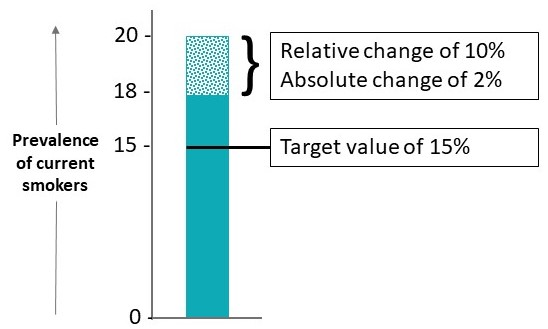
\includegraphics{Scenario-Abs, Rel, Target cropped} 

}

\caption{Comparison of health intervention scenario types}\label{fig:unnamed-chunk-10}
\end{figure}

To adjust the prevalence of smokers, the change is applied to every
current smoker in the population; individuals are not selected at
random. \ldots{}.

\section{Scenario: Cause-deleted}\label{scenario-cause-deleted}

What would be the life expectancy of a population if be no one in the
population ever smoked? This scenario is a cause-deleted scenario.

There are two distinct terms in cause-deleted calculations:

\begin{itemize}
\item
  \textbf{Cause-deleted life expectancy} is the estimated life
  expectancy for the counterfactual population where a specific cause
  (e.g.~smoking) never existed. E.g. the counterfactual population was
  always never smokers.
\item
  \textbf{Cause-deleted effect of life expectancy} or \textbf{life years
  lost due to the cause} is the full effect of the cause (e.g smoking)
  in the population. E.g. In a population 3 years of life are lost due
  to individuals in that population smoking: either currently or
  previously.
\end{itemize}

If multiple causes are selected (e.g.~smoking and physical inactivity)
the cause-deleted life expectancy calculated accounts for both of these
effects and the cause-deleted effect of life expectancy (or life years
lost) is calculated for each individual cause.

\textbf{Note:}
\(\text{Cause-deleted life expectancy of smoking and physical inactivity} \neq\)
\(\text{Cause-deleted effect of smoking} + \text{Cause-deleted effect of physical inactivity}\)

This is because individuals in the population may be both smokers and
physically inactive.

\emph{Insert table with the reference levels for each of the health
behaviours}

\subsection{Cause-deleted calculation}\label{cause-deleted-calculation}

There are two parts to the calculations preformed in cause-deleted
scenarios: (A) calculate the risk, and (B) calculate the health outcome:
life expectancy or number of deaths.

\textbf{Part A: Risk calculations}

The original multivariable predictive risk algorithm is:

\[ \text{Risk} = \sum_t h_0(t) * e^{\beta_{pred.smoking}*x_{smoking}+\beta_{pred.cancer}*x_{cancer} + \beta_{pred.age}*x_{age} +...}  \]

\textbf{Step 1.} Modify the original algorithm to include the external
coefficient(s). This means replacing all predictive hazard ratios/betas
related to the health behaviour to the causal hazard ratios/betas.

\begin{itemize}
\tightlist
\item
  Remove the original regression coefficient(s) for the health
  behaviour.
\item
  Add the new external coefficient(s) to the algorithm. External
  coefficients are generated from either: causal models, or from
  systematic reviews or meta-analysis.
\end{itemize}

\[ \text{External coefficient risk} = \sum_t h_0(t) * e^{{\beta_\textbf{causal.smoking}}*x_{smoking} + {{\beta_\textbf{causal.cancer}}}*x_{cancer} + \beta_{pred.age}*x_{age} +...}  \]

\textbf{Step 2.} Risk is calculated using the modified algorithm created
in Step 1 and the respondent's original profile (e.g.~current smoker).
This is the ``external coefficient risk''.

\[ \text{External coefficient risk} = \sum_t h_0(t) * e^{\beta_{causal.smoking}* {(\textbf{current smoker})} + \beta_{causal.cancer}*x_{cancer} + \beta_{pred.age}*x_{age} +...}  \]

\textbf{Step 3.} ``Cause-deleted risk''' is calculated by setting an
exposure to a reference (non-exposed) value (all other risk exposures
remain unchanged).

\[ \text{Cause-deleted risk' } = \sum_t h_0(t) * e^{\beta_{causal.smoking}* {(\textbf{never smoker})} + \beta_{causal.cancer}*x_{cancer} + \beta_{pred.age}*x_{age} +...}  \]

\textbf{Step 4.} The ``cause-deleted effect external'' is calculated as
``external coefficient risk'' (Step 2) minus the ``cause-deleted
risk'.''(Step 3).

\[\text{Cause-deleted effect}_{external} = \text{External coefficient risk} - \text{Cause-deleted risk'}\]

\textbf{Step 5.} Original risk is calculated using the original
algorithm and the original respondent's profile.

\[ \text{Original risk} = \sum_t h_0(t) * e^{{\beta_\textbf{pred.smoking}}*{(\textbf{current smoker})}+{\beta_\textbf{pred.cancer}}*x_{cancer} + \beta_{pred.age}*x_{age} +...}  \]

\textbf{Step 6.} The ``cause-deleted risk external'' is calculated by
``original risk'' (Step 5) minus the ``cause-deleted effect external''
(Step 4).

\[\text{Cause-deleted risk}_{ external} = \text{Original risk} - \text{Cause-deleted effect}_{external}\]

\begin{figure}

{\centering 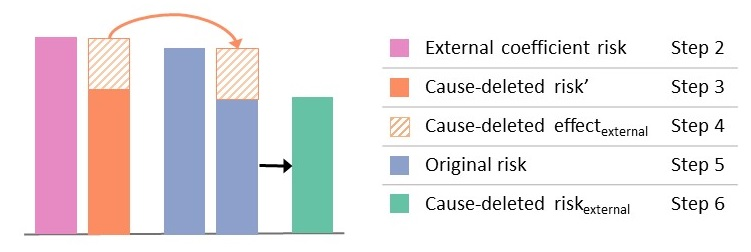
\includegraphics{Method2 only -cbf} 

}

\caption{Risk portion of the cause-deleted calculations}\label{fig:unnamed-chunk-11}
\end{figure}

\textbf{Part B: Health outcome calculations}

Using risks generated above you can then calculate:

\begin{itemize}
\tightlist
\item
  cause-deleted life expectancy or life years lost attributable to a
  health behaviour (exposure)
\item
  cause-deleted number of deaths or number of deaths attributable to a
  health behaviour (exposure)
\end{itemize}

\textbf{Life expectancy calculations}

Step I: Calculate the original life expectancy by using the original
risk (Step 5 above) in the sex-specific 5-year abridge period life
tables.

Step II: Calculate the cause-deleted life expectancy by using the
cause-deleted risk external (Step 6 above) in the sex-specific 5-year
abridge period life tables.

Step III: Calculate life years attributable to a health behaviour by:
original life expectancy (Step I) minus cause-deleted life expectancy
(Step II):

\[ \text{Life years due to exposure} = \text{Original life expectancy} - \text{Cause-deleted life expectancy}\]
If the life years attributable to a health behaviour are negative then
the value represents the life years lost due to smoking.

\textbf{Number of deaths calculations}

Step I: Calculate the number of deaths that would occur using the
original risk (Step 5 above).

Step II: Calculate the number of deaths that would occur using the
cause-deleted risk external (Step 6 above).

Step III: Calculate the number of deaths that are attributable to a
health behaviour (exposure) by: original number of deaths (Step I) minus
cause-deleted number of deaths (Step II):

\[\text{Deaths due to exposure} = \text{Original number of deaths} - \text{Cause-deleted number of deaths}\]

\section{Limitations}\label{limitations}

\chapter{Glossary}\label{glossary}

\textbf{5-year mortality risk}

The probability that an individual will die in the next 5 years.

\textbf{Body Mass Index (BMI)}

A weight-to-height ratio used as an indicator of obesity and
underweight. BMI is calculated by dividing an individual's body weight
in kilograms by the square of height in metres (kg/m2).

\textbf{Burden}

The impact or size of a health problem in an area, measured by cost,
mortality, morbidity or other indicators. The burden of unhealthy
behaviour is calculated by the differences in life expectancy based on
individuals' exposure to four health behavioural risks for poor health
relative to the healthy category.

\textbf{By Row Measures}

When selected, the result will be the measurement for
each individual (e.g.~row) in the dataset.

\textbf{Calibration}

The agreement between predicted risk generated from the model and
observed risk generated from the data.

\textbf{Canadian Community Health Survey}

An annual survey preformed by Statistics Canada that collects
information related to health status, health care utilization and health
determinants for the Canadian population. Details about the survey can
be found on Statistic Canada website
(\url{http://www23.statcan.gc.ca/imdb/p2SV.pl?Function=getSurvey\&Id=144170}).

\textbf{Cause-deleted life expectancy}

A cause-deleted health outcome is the estimated
health outcome of a population if a specific cause (e.g.~smoking) did
not exist in that population.

\textbf{Discrimination}

The ability of the model to differentiate between high risk individuals
and low risk individuals.

\textbf{Error Message}

Error messages will occur when variables that are
\textbf{``Required for Calculation''} are missing in the data. If the
entire column for the variable is missing then the calculation cannot be
performed on the data. If there are missing row entries for the variable
then the entire row will not be used in the calculation.

\textbf{Filter}

Chooses part of your dataset for analysis. If you filter on
`Sex' and then `Male', calculations will only be performed on
individuals that are `Male' and `Females' will be excluded. For example,
when calculating Life Expectancy on the filter variable `Sex' then
`Male' there will be a Life Expectancy estimate for `Males' and
\emph{no} Life Expectancy estimate for `Females'.

\textbf{Health Behaviour}

Actions people do that may affect their health, positively or
negatively. Health behaviours are among the determinants of health and
are influenced by the social, cultural and physical environments in
which people live and work.\citep{StatsCan2010} They are also shaped by
individual choices and external constraints.\citep{StatsCan2010} The
four health behaviours of \textbf{smoking, alcohol consumption, diet,}
and \textbf{physical activity} are specified in Project Big Life's
planning tool.

\textbf{Ignored Variables}

Are not included in the calculation. It does not matter if your dataset
includes these variables or not. Ignored variables can used for filter
and stratification.

\textbf{Life Expectancy (LE)}

Life expectancy is a calculation of how long a person or
population would be expected to live, on average, given unchanging risk
of death from a specific point in time.

\textbf{Metabolic Equivalent of Task (MET)}

The metabolic equivalent of task (MET) is a measure of the rate of
energy expenditure from an activity; a measure of calories burned by
type, duration and frequency of physical activity. The reference value
of 1 MET is defined as the energy expediture rate at rest which is equal
to 1kcal/kg/day.

\textbf{Predictor}

A variable that is used in the algorithm to predict the outcome.

\textbf{Recommend for calculation}

Variables that are included in the calculation but not necessary for the
calculation to run. Rather these variables increase the accuracy of the
results.

\textbf{Required for calculation}

Variables that are included in the calculations and are necessary for
the calculation to run. If a dataset does not have these variables then
the calculation will not run.

\textbf{Risk}

The probability ofa health event occuring at some point of time in the
future.

\textbf{Socioeconomic Position}

People in poorer socioeconomic circumstances generally have poorer
health. Deprivation measures identify those who experience material or
social disadvantage compared to others in their community. The
Deprivation Index for Health in Canada developed by the Institut
national desanté publique du Québec (INSPQ)\citep{INSPQ2000} is used in
this plannning tool. The index includes education, employment and income
as measures of material deprivation; and single-parent families, living
alone, or being divorced, widowed or separated as measures of social
deprivation. The deprivation index was used to assign geographical areas
into socioeconomic position groups (low, middle and high) based on
material and social quintiles. High-deprivation neighbourhoods were
those in the top two quintiles for both social and material deprivation.
Low-deprivation neighbourhoods were those in the bottom two quintiles.

\textbf{Stratification}

The seperation of data into smaller strata (levels or
classes which individuals are assigned too). If the variable `Sex' is
stratified it creates two strata: `Male' and `Female'. Calculations are
performed on each strata (level or class) and the outcome will be
specific to that strata. For example, when calculating Life Expectancy
on the stratified variable `Sex' there will be a Life Expectancy
estimate for `Males' and a different Life Expectancy estimate for
`Females'.

Stratification can only occur on categorical variables.

\textbf{Summary Measures}

When selected, the result will be a single measure for
the entire dataset. For instance when Summary Measure - Life Expectancy
(Summary Measure) is selected the result is a single life expectancy for
the given for the population.

When stratifications are selected, the summary
measure will be given for each strata. For instance when Summary Measure
- Life Expectancy and Stratification - Sex are selected, then two life
expectancy measures will be given one for males and one for females.

\textbf{Warning Message}

Warning messages will occur when variables that are
\textbf{``Recommended for Calculation''} are missing in the data. If the
entire column for the variable is missing the calculation will still be
performed on the data. If there are missing row entries for the variable
the row will still be used in the calculation


















































\appendix


\chapter{Mortality Population Risk Tool
(MPoRT)}\label{mortality-population-risk-tool-mport}

\textbf{Outcomes: 5-yr risk of death, Life Expectancy, Cause-deleted
Life Expectancy}

\textbf{Calculations}

Using MPoRT you are able to calculate:

\begin{itemize}
\tightlist
\item
  5 year mortality risk
\item
  Number of deaths
\item
  Life Expectancy
\item
  Cause-deleted deaths and life expectancy
\item
  Burden of health behaviour in deaths and on life expectancy
\end{itemize}

\textbf{Types of Questions}

\begin{itemize}
\tightlist
\item
  What is the burden of smoking on life expectancy?
\item
  How many deaths would be prevented if everyone met their daily
  excercise requirements?
\end{itemize}

\textbf{Description}: A multivariable predictive risk model that
estimates the future risk of all-cause death in Canada. It adjusts for
health behaviours: smoking, unhealthy alcohol consumption, poor diet,
and physical inactivity, and a wide range of other risk factors.

Versions of MPoRT have been developed since 2012 and used in various
studies. Each version of MPoRT (v1.0, v1.2, v2.0) used the Ontario
subset of the Canadian Community Health Survey (CCHS) for development
and the survey respondents were linked to personal death records. In
later versions of MPoRT (v1.2, v2.0) the following changes were made:,
(a) algorithm variables were adjusted to improve predictions, and (b)
the algorithms were validated using: the Ontario subset of CCHS of the
years that were not used in development and the National CCHS dataset
(excluding Ontario).

\textbf{MPoRTv1.0} Was used in the ``Seven More Years'' report, a joint
report with Public Health Ontario and IC/ES
(\url{https://www.ices.on.ca/Publications/Atlases-and-Reports/2012/Seven-More-Years}).
In summary, the algorithm estimated the risk of death associated with
health behaviours: smoking, unhealthy alcohol consumption, poor diet,
physical inactivity and stress. There were approximately 550,000
person-years of follow up and over 6000 deaths in the development
dataset. The algorthim used categorical predictor variables for health
behaviours and sociodemographic factors.

\textbf{MPoRTv1.2} Was published in PLoS
(\url{https://journals.plos.org/plosmedicine/article?id=10.1371/journal.pmed.1002082}).
In summary, the algorithm estimated the risk of death associated with
health behaviours: smoking, unhealthy alcohol consumption, poor diet,
and physical inactivity (stress was removed due to its low prediction
ability). There were approximately 1 million person-years of follow up
and over 9000 deaths in the development and validation datasets. The
algorithm used multiple continous predictor variables, and added chronic
disease predictor variables and interaction terms.

\textbf{MPoRTv2.0 - The version used in Project Big Life's Planning
Tool} This version of MPoRT has not yet been published.

\emph{Development}: This predictive risk model was developed using
Ontario subsets of the 2001 to 2008 CCHS and participants were linked to
personal health records. There were approximately 1.3 million
person-years of follow-up and over 15,000 deaths in the developmental
dataset.

\emph{Validation}: This predictive risk model was validated using three
different datasets: Ontario subset of the 2009 to 2012 CCHS, National
dataset (except Ontario) of the 2003 to 2008 CCHS, and the National
dataset of the 2000 and 2005 National Health Interview Survey in the
United States of America. In all validation datasets individuals were
linked to personal health records.

\emph{Parameters}: The parameters used in this predictive risk model
are:

Category

Variable

Scale

Description

Demographic

Age*

Continous

5 knot spline. Valid range 20 to 102

Sex

Dichotomous

Stratified Female/Male

Health Behaviour

Pack years of smoking

Continous

3 knot spline. Valid range: 0 to 78 (Female), 0 to 112.5 (Male)

Smoking Status

Categorical

Non-smoker

Current Smoker

Former Smoker \textless{}= 5 years

Former \textgreater{} 5 years

Alcohol (number of drinks per week)

Continous

4 knot spline (Females) and 3 knot spline (Males). Valid range: 0 to 25
(Female), 0 to 50 (Male)

Former/non-drinker

Dichotomous

Yes/No

Simplified diet score

Continous

3 knot spline. Valid range: -18.9 to 20.7 (Female), -16.8 to 18.4 (Male)

Leisure physical activity (MET)

Continous

3 knot spline. Valid range: 0 to 12.4 (Female), 0 to 16 (Male)

Socio-demographic

Ethnicity

Categorical

White

Black

Chinese

Arab; South Asian; West Asian

Filipino; Japanese; Korean; Southeach Asian

Other; Indigenous; Latin American; Multiple origin; unknown

Immigrant

Dichotomous

Yes/No

Fraction of lifetime in Canada

Continous

3 knot spline\textsuperscript{†}. Valid range: 0 to 1

Education

Categorical

Less than secondary

Secondary School Graduation

Some Post-Secondary

Post-Secondary Graduation

Neighbourhood social and material deprivation

Ordinal

Low (1st or 2nd quantile

High (4th or 5th quantile)

Moderate (all others)

Chronic Conditions

Diabetes

Dichotomous

Yes/No

High Blood Pressure

Dichotomous

Yes/No

Chronic Respiratory Disease

Dichotomous

Yes/No

Mood Disorder

Dichotomous

Yes/No

Cancer

Dichotomous

Yes/No

Dementia

Dichotomous

Yes/No

Heart Disease

Dichotomous

Yes/No

Stroke

Dichotomous

Yes/No

Epilepsy

Dichotomous

Yes/No\textsuperscript{‡}

BMI

Continous

3 knot spline. Valid range: 8.9 to 47.2 (Female), 8.6 to 43.7 (Male)

* Age interaction included for all variables exept immigrant, fraction
of time in Canada, and ethnicity † Excluded in the male model, remains
in the female model ‡ Excluded in the female model, remains in the male
model

\bibliography{book.bib,packages.bib}


\end{document}
